\documentclass[11pt,a4paper]{report}

% part of template
\usepackage{url}
\usepackage[utf8]{inputenc}
\usepackage{graphicx}
\usepackage[all]{xypic}
\usepackage{amsmath}
\usepackage{amsthm}
\usepackage{array}
\usepackage{todonotes}
\usepackage{listings}
\usepackage[a4paper]{geometry}

% my packages
% \usepackage{minted}
\usepackage{biblatex}
\usepackage{amssymb}
\addbibresource{bib/thesis.bib}

\theoremstyle{definition}
\newtheorem{defn}{Definition}[section]

\def\ci{\perp\!\!\!\perp}
% \def\space{\!\!\!}
\lstset{language=Python}

\makeatletter %otherwise geometry resets everything
\Gm@restore@org
\makeatother

\setlength{\itemsep}{0cm}
\setlength{\voffset}{0cm}
\setlength{\headheight}{0cm}
\setlength{\topmargin}{0cm}
\setlength{\extrarowheight}{3pt} %for superscripts in tabular
\setlength{\arraycolsep}{4pt}
\lstset{basicstyle = \footnotesize, breaklines = true}

\graphicspath{{imgs/}}

\begin{document}
\begin{titlepage}
\begin{center}
\textsc{\LARGE Bachelor thesis\\Computing Science}\\[1.5cm]

\includegraphics[height=100pt]{logo}

\vspace{0.4cm}
\textsc{\Large Radboud University}\\[1cm]
\hrule
\vspace{0.4cm}
\textbf{\huge Bayesian Constraint-based Causal Discovery with Greedy
  Search}\\[0.4cm]
\hrule
\vspace{2cm}
\begin{minipage}[t]{0.45\textwidth}
\begin{flushleft} \large
\textit{Author:}\\
Daan Spijkers\\
s1011382
\end{flushleft}
\end{minipage}
\begin{minipage}[t]{0.45\textwidth}
\begin{flushright} \large
\textit{First supervisor/assessor:}\\
dr. Tom Claassen \\
\texttt{tomc@cs.ru.nl}\\[1.3cm]
% \textit{[Second supervisor:]}\\
% title, name\\
% \texttt{e-mail adress}\\[1.3cm]
\textit{Second assessor:}\\
title, name\\
\texttt{e-mail adress}
\end{flushright}
\end{minipage}
\vfill
{\large \today}
\end{center}
\end{titlepage}

\listoftodos
% The abstract of your thesis is a brief description of the research hypothesis,
% scientific context, motivation, and results.
% The preferred size of an abstract is one paragraph or one page of text.
\begin{abstract}
How much can we improve the accuracy of the resulting PAG from the BCCD
algorithm using a greedy MAG search to optimise its probabilistic causal
statements?
\todo{abstract is not written properly}
\end{abstract}

\tableofcontents

% The introduction of your bachelor thesis introduces the research area, the
% research hypothesis, and the scientific contributions of your work.
% A good narrative structure is the one suggested by Simon Peyton Jones
% \begin{itemize}
% \item describe the problem / research question
% \item motivate why this problem must be solved
% \item demonstrate that a (new) solution is needed
% \item explain the intuition behind your solution
% \item motivate why / how your solution solves the problem (this is technical)
% \item explain how it compares with related work
% \end{itemize}
% Close the introduction with a paragraph in which the content of the next chapters
% is briefly mentioned (one sentence per chapter).
\chapter{Introduction}\label{introduction}
Causal inference consists of taking a system of statistical
independencies, and mining a system of causal relations. These causal
relations we then represent in a causal graph.

In an ideal situation, we have a statistical test that determines
whether $X$ and $Y$ are independent with 100\% accuracy. Given such a
perfect test, complete algorithms exist; they give the total causal
information possible from that system. Unfortunately, in the real world
100\% accuracy is not possible, and we often have to make do with
insufficient data.

That is why taking realistic data, and optimizing the result is a relevant
problem. It is not always clear how an algorithm performs in these
situations, even if it is complete. One such complete algorithm is
BCCD\cite{claassenBayesianApproachConstraint2012}, which uses a bayesian
score to return a more robust and informative result than comparable
procedures.

BCCD uses a score-based method to mine a system of logical statements of
the following form:
\begin{align*}
  X \Rightarrow Y \lor X \Rightarrow Z \\
  X \not \Rightarrow Y \land X \not \Rightarrow Z
\end{align*}
That is: information about cause or non-cause between different stochastic
variables. These statements have a particular accuracy associated with
them, representing how sure BCCD is about it. BCCD then uses causal
inference to deduce statements that can be mapped into a PAG. However,
since the data can contain inconsistencies, so can the statements. As of
currently, the way inconsistencies are solved is by using statements in
ascending accuracy, thereby never overwriting information we are more sure
of.

However, it is quite possible that one higher accuracy statement, say
$p_1 = 0.9$ is contradicted by two slightly lower accuracy statements,
say $p_2, p_3 = 0.85$. A simple estimation the likelihood of these
situations is:
\begin{align*}
  p_1 * (1 - p_2) * (1 - p_3) &= 0.9 * (1 - 0.85) * (1 - 0.85) &= 0.02 \\
  (1 - p_1) * p_2 * p_3 &= 0.1 * 0.85 * 0.85 &= 0.07
\end{align*}
It is clear then, that we would rather have the second situation, where
the two lower accuracy statements are true, and that there is something to
be gained here.

An initial impulse is to improve the outcome by cleverly choosing which
statements we do use to construct the graph, and which we do not. This
ends up being a very difficult problem however, and instead we will work
the other way around. That is, by starting at the graph.

We take the initial output of BCCD, as well as its logical statements, and
then iteratively search for better graphs until there is no further
improvement possible. Although doing this greedily means this is likely to
end up in a local optimum, the score must end up higher or equal to the
initial BCCD result.

By doing this we will be using global information to complement the local
information, hopefully getting a better result. To easy scoring we will
first convert the BCCD PAG to a MAG, and then work on that MAG. As we will
see, this conversion also improves the result significantly, presumably
because this incorporates global information that the original algorithm
did not.

To summarize, our contributions are as follows:
\begin{enumerate}
  \item An improved result on the BCCD framework by converting to and from
    a MAG.

  \item A greedy step which takes the MAG and BCCD statements, and returns
    a higher scoring MAG.
\end{enumerate}

% This \emph{optional} chapter contains the stuff that your reader needs
% to know in order to understand your work. Your ``audience" consists of
% fellow third year computing science bachelor students who have done the
% same core courses as you have, but not necessarily the same
% specialization, minor, or free electives.
\chapter{Preliminaries}\label{preliminaries}
\section{Causal Discovery by Example}\label{sec:example}

% TODO(daan): explain what a DAG is, then we move on to the example

In this section we will give a quick introduction to causal discovery. To
do so, similar to \cite{zhangCompletenessOrientationRules2008}, we use the
example from \cite{richardsonChainGraphsSymmetric1998}, which is
attributed to Chris Meek:

\begin{quote}
  The graph (figure \ref{fig:example}) represents a randomized trial of an
  innefective drug with unpleasant side-effects. Patients are randomly
  assigned to the treatment or control group (A). Those in the treatment
  group suffer unpleasant side-effects (Ef), the severity of which is
  influenced by the patient's general level of health (H), with sicker
  patients suffering worse side-effects. Those patients who suffer
  sufficiently severe side-effects are likely to drop out of the study.
  The selection variable (Sel) records whether or not a patient remains in
  the study, thus for all those remaining in the study Sel=StayIn. Since
  unhealthy patients who are taking the drug are more likely to drop out,
  those patients in the treatment group who remain in the study tend to be
  healthier than those in the control group. Finally health status (H)
  influences how rapidly the person recovers (R).
\end{quote}

\begin{figure}
  \centering
  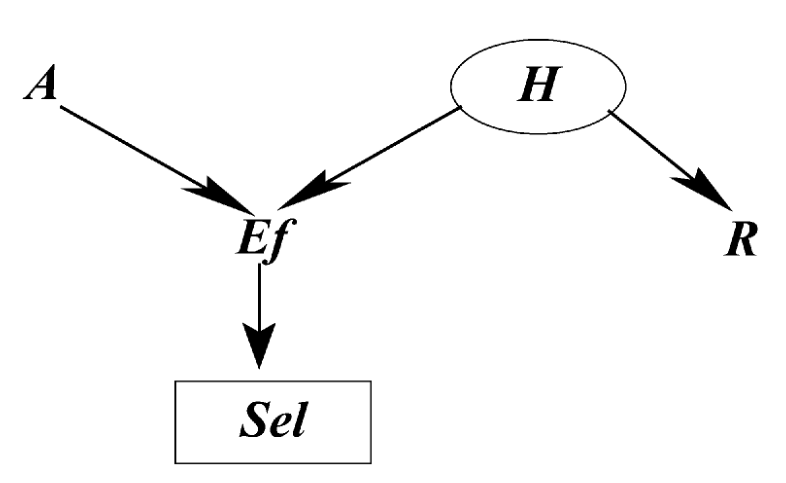
\includegraphics[width=0.5\textwidth]{imgs/example1.png}
  \caption{Example showing both latent cofounders and selection variables.}
  \label{fig:example}
\end{figure}

In this study we would like to describe the relation between recovery (R),
treatment (A), and side-effects (Ef). But as we see, it is also influenced
by the health (H) of the patient, and whether they semain in the study
(Sel). In this case health is a \emph{latent cofounder} and Sel is a
\emph{selection variable}. In a normal DAG there is no way to represent
these without knowing their existence, so we will introduce a mixed graph
called an Ancestral Graph. We introduce undirected and bidirected edges,
and change the meaning of marks in the following way:

\begin{itemize}
  \item $A \rightarrow B$ means A causes B or some selection variable, and B
    does not cause A or a selection variable.

  \item $A \leftrightarrow B$ means A does not cause B or a selection
    variable, and B does not cause A or a selection variable.

  \item $A - B$ means A causes B or a selection variable, and B causes A
    or a selection variable. As we shall see in
    \ref{sec:ancestral_graphs}, this must mean that both A and B cause
    some selection variables.
\end{itemize}

In the case that there is no selection bias, we have no undirected edges,
and $A \rightarrow B$ means A causes B. We then are only left with $A
\leftrightarrow B$, meaning a latent cofounder.
\todo{explain somewhere that an edge means relation, which is why latent
cofounder}

\section{d-seperation}
Although we have introduced what causal graphs are, we have not yet shown
the relation between a graph and statistical independencies. Given that
that is what (constraint-based) discovery is about, it would be prudent to
at least define it.

In a causal graph, there is no edge $A \rightarrow B$ if $A$ and $B$ are
d-seperated.

% TODO(daan): add description of d-seperation
\begin{defn}
  X is conditionally independent of Y given a collection of variables Z,
  denoted $X \ci Y | Z$ iff there is no unblocked path between X and Y in
  G conditional on the nodes in Z.
\end{defn}

\begin{defn}
  Causal Markov Condition states that each variable is indipendent of its
  non-descendants, given its parents.
\end{defn}

\begin{defn}
  Causal Faithfulness Conditional states that there are no independencies
  between variables that are not entailed by the causal markov condition.
\end{defn}


\section{Ancestral Graphs}\label{sec:ancestral_graphs}
Although we now have introduced the meaning of ancestral graphs, we have
not yet defined what it means to have valid MAGs or PAGs.

MAG is a maximal ancestral graph, with no almost directed cycles.
% TODO(daan): fix description of MAG and PAG

PAG is the equivalence class of a MAG.

% This chapter, or series of chapters, delves into all technical details
% that are required to \emph{prove} your scientific hypothesis. It should
% be sufficiently detailed and precise in order for any fellow computing
% scientist student to be able to \emph{repeat} your research and
% therewith establish the same results / conclusions that you have
% obtained. Please note that, in order to improve readability of your
% thesis, you can put a part of this information also in one or more
% appendices (see Appendix \ref{appendix}).
\chapter{Algorithm Overview}\label{algorithm}
Our procedure turns out to be very simple, and we shall see that the most
challenging part is scoring the graph, which we get into in section
\ref{checking}. For now we shall give a short overview of the algorithm,
and then go into more detail on each of the problems. We give Python-esque
pseudocode:

% TODO(daan): improve pseudocode formatting
\begin{lstlisting}
def bccdgs(pag, statements):
    mag = pag_to_mag(pag)
    next_mag = next_mag(mag)

    while score(next_mag, statements) > score(mag, statements):
      mag = next_mag
      next_mag = next_mag(next_mag)

    return mag_to_pag(mag)
\end{lstlisting}
Where we use one helper function:
\begin{lstlisting}
def next_mag(mag, statements):
    adjacent_mags = adjacent_mags(mag)
    return best_scoring_mag(mags, statements)
\end{lstlisting}
We see that the first thing we do is convert the PAG into a MAG, since
scoring a MAG is easier. Then, within the while loop we keep looking for
the best adjacent mag with the next\_mag function. Within this function we
generate adjacent mags, and then pick the best scoring one. In short,
there are 4 main problems to solve:
\begin{enumerate}
  \item Transforming a PAG into a MAG.

  \item Transforming a MAG into a PAG.

  \item Generating adjacent MAGs.

  \item Scoring a MAG.
\end{enumerate}
We will handle these problems in the following sections.

\section{PAG to MAG}
To turn a PAG into a MAG we have to change all circle marks into either
tails or arrows. However, we must be careful that the MAG is a part of the
equivalence class. A proven correct method is as follows:

\begin{enumerate}
  \item Turn all semi-arcs into arcs. That is, turn
    $*\!\!\!\rightarrow$ into $\rightarrow$ and
    $*\!-$ into $\leftarrow$.

  \item Orient the remaining $*\!\!\!-\!\!\!*$ edges into a DAG with no new unshielded
    colliders.
\end{enumerate}
It is clear that all circle edges are either arrows or tails. For the
proof that this is a valid MAG from the correct equivalence class we refer
to the original paper\cite{zhangCompletenessOrientationRules2008}.

\section{MAG to PAG}
Turning a MAG back into a PAG is slightly more involved, as it is not
clear which marks must turn into circles. We do not have an algorithm that
works directly on a MAG, and instead we will use d-seperation to determine
independencies. We then feed this into the FCI algorithm, and make use of
its orientation rules. Since the rules are complete and sound, this will
create a PAG of the correct equivalence class.

\section{Adjacent MAGs}
\subsection{Generating}
This is the simplest problem to solve. We consider adjacent graphs to be
graphs which have one edge changed compared to the original. Given two
vertices $u$ and $v$, there are four possibilities:
\begin{align}
  u \rightarrow v \\
  u \leftarrow v \\
  u \leftrightarrow v\\
  (u, v) \notin E
\end{align}
Remembering that we ignored selection bias, and so there are no undirected
edges. Our original graph has one of these four. All adjacent MAGS can
then be easily generated by adding a graph which has one of the other 3
possibilities.

The real issue comes up when we want to check whether this MAG is also
valid; that is whether it has any almost directed cycles.

\subsection{Checking correctness}\label{transitive_closure}
We want to check that \emph{for any directed path from $u$ to $v$, there
does not exist an edge $u \leftarrow v$ or an edge $u \leftrightarrow v$.
} To do this, we will check a graph of all directed paths, the transitive
closure, and compare it to the original graph.

Although an efficient algorithm of $O(|V||E|)$ exists
\cite{purdomTransitiveClosureAlgorithm1970} and is implemented in the
boost graph library \cite{siekBoostGraphLibrary2002}, using this library
in Python is a bit of a hassle. Instead, we use a simple algorithm based
on matrix multiplication. This has $O(|V|^4)$, but the implementation is
optimized enough for our purposes, as we shall discuss in section
\ref{runtime}.

The definition of arbitrary matrix multiplication for $C = A \cdot B$ is:

\begin{equation*}
  c_{ij} = \sum ^n_{k=1} a_{ik}b_{kj}
\end{equation*}

Now for an adjacency matrix $A \in \mathbb{B}^{n \times n}$ the
self-product $A \cdot A$ becomes:

\begin{equation*}
  a^2_{ij} = \sum ^n_{k=1} a_{ik}a_{kj}
\end{equation*}

So we see that $a^2_{ij} > 0$ iff there is some directed path from $i$ to
$j$ of length 2. Now if we want the transitive closure we take $A^n$, as a
directed path is of maximum length $n$.

Now that we have the transitive closure we can easily check whether any
directed paths exist by comparing $A^n$ to $A$.

\section{Checking}\label{checking}
Although we build on the BCCD algorithm, it is quite complex, and details
on how it works are outside of the scope of this thesis. Instead, we will
focus on the output we use from it, which is the logical statements. For
the interested reader, we refer to the original paper on how they are
generated\cite{claassenBayesianApproachConstraint2012}.

Given that we ignore selection bias, the specific different logical
statements are as follows:
\begin{align*}
  X &\Rightarrow Y \\
  X \Rightarrow Y &\lor X \Rightarrow Z \\
  X \not \Rightarrow Y &\land X \not \Rightarrow Z \\
  (X, Y) &\notin E \\
  X &\ci Y
\end{align*}
We see that besides information about cause and non-cause, we now also
have information about the non-existence of an edge, and unconditional
independence of variables.

Besides the graph $G$ we will also need its transitive closure $G_{tc}$ to
check whether an arbitrary statement $s \in S$ is true. We use the
algorithm discussed in section \ref{transitive_closure}. Given this
transitive closure, checking (non-)cause and edge existence is incredibly
easy. For $X \Rightarrow Y$ we check $(X, Y) \in E_{tc}$, and $X \not
\Rightarrow Y$ similarly $(X, Y) \notin E_{tc}$. The only statement which
requires some work is unconditional independence.

\todo{change to a consistent notation for directed path}
There are 3 cases in which $X \not \ci Y$:
\begin{enumerate}
  \item $(X, Y) \in E_{tc}$ or $(Y, X) \in E_{tc}$

  \item $X \leftrightarrow Y$

  \item There exists a $Z$ such that $X \leftarrow \ldots \leftarrow Z
    \rightarrow \ldots \rightarrow Y$
\end{enumerate}
These can all easily be checked with $G$ and $G_{tc}$.

\section{Scoring}\label{sec:scoring}
To create a concrete score from these statements we have to combine the
accuracies in some way. To do this we assume that these statements are
independent. This is patently untrue, but we need this assumption to
combine them easily.

Now we can describe the probability of a graph $G$ given statements $S =
\{s_1, \ldots, s_l\}$ as follows:
\todo{fix notation of p i}

\begin{equation*}
  \mathbb{P}(G | S) = \prod ^l_{i=1} p_i
\end{equation*}

Maximizing this is equivalent to maximizing the log-likelihood, which is
what we will do:

\begin{equation*}
  L(G|S) = \sum_{i=1}^l \log (p_i)
\end{equation*}

To find the best graph from a collection we then take the graph which
maximizes this score.

\section{Implementation details}
Now that all the pieces are there we give a quick overview of what we used
to implement them. We primarily used the Python package Numpy
\cite{harrisArrayProgrammingNumPy2020} to represent graphs as an adjacency
matrix. Besides that, the following packages were used:
\begin{itemize}
  \item RUcausal \todo{add rucausal link} for the BCCD implementation.

  \item Pcalg\cite{kalischCausalInferenceUsing2012} for pag2mag and fci
    functions. It is also used to generate random graphs, as we shall see
    in chapter \ref{results}.

  \item Scipy\cite{virtanenSciPyFundamentalAlgorithms2020} for the matrix
    power used in \ref{transitive_closure}.

  \item Seaborn\cite{waskomSeabornStatisticalData2021} and
    Matplotlib\cite{hunterMatplotlib2DGraphics2007} for plotting results.

  \item The rpy2 package to call R packages from Python.
\end{itemize}

\chapter{Experiments}\label{results}

\section{Setup}
We use pcalg to generate random graphs. Unless otherwise noted, the
expected node degree is 2.5, and each graph has 10 nodes. We generate 100
random DAGs, and then from each graph we generate $2^7, \ldots, 2^{17}$
samples, and run the algorithm on those samples.

By bccd we mean the PAG output from bccd, bccmp is the PAG converted to a
MAG, and then converted to a PAG again. bccdgs is bccdmp with the greedy
search added.

We will look at the performance of each algorithm for different graph
size and different graph densities. We will also look at what the best
parameters for bccdgs are.

\section{Algorithm results}

\todo{All plots need to be finalized with proper captions, etc}
\subsection{Graph size}
The first comparison is of the different algorithms on several graph
sizes, shown in figure \ref{fig:nodes_causal}. While the 3 algorithms are
roughly equivalent for graphs of 5 nodes, we do see significant
differences in 10 and 15 nodes. It is immediately clear that both bccdmp
and bccdgs outperform bccd by a significant margin.
\begin{figure}
  \centering
  \includegraphics[width=\textwidth]{lib/nodes_pag.pdf}
  \includegraphics[width=\textwidth]{lib/nodes_causal.pdf}
  \caption{Graph size}
  \label{fig:nodes_causal}
\end{figure}

\subsection{Graph density}
We can plot similar results for different density graphs. Although we
might have guessed that bccdgs works better than bccdmp for more difficult
problems, e.g. larger or denser graphs, it does not appear to directly be
the case here. We see that for degree=3 bccdgs does not outperform bccdmp
consistently, and in fact underperforms for lower amount of samples.
\begin{figure}
  \centering
  \includegraphics[width=\textwidth]{lib/density_pag.pdf}
  \includegraphics[width=\textwidth]{lib/density_causal.pdf}
  \caption{Density}
  \label{fig:density_causal}
\end{figure}

\section{Parameters}
There are three main parameters we want to check, that is whether to keep
the skeleton, what value to take for k, and which accuracy statements to
include.

\subsection{Skeleton}
The skeleton concerns how we generate new graphs. This is similar to what
BCCD does, which is keep the skeleton from the constraint-based method,
and map the orientation gathered by the statements on top of it. As we see
in figure \ref{fig:skel_causal}, keeping the skeleton the same gives a
better result.
\begin{figure}
  \centering
  \includegraphics[width=0.33\textwidth]{lib/skel_pag.pdf}
  \includegraphics[width=0.33\textwidth]{lib/skel_causal.pdf}
  \caption{Skeleton}
  \label{fig:skel_causal}
\end{figure}

\subsection{k}
Besides generating all graphs with one edge different, we can also choose
to change 2 edges. Although we would expect this to give a better result,
the result actually ends up worse, as shown in figure \ref{fig:k_causal}.
We are not sure what caused this.
\begin{figure}
  \centering
  \includegraphics[width=0.33\textwidth]{lib/k_pag.pdf}
  \includegraphics[width=0.33\textwidth]{lib/k_causal.pdf}
  \caption{k}
  \label{fig:k_causal}
\end{figure}

\subsection{Cutoff}
Probably the most interesting paramater is the cutoff point for what
probability statements to include. Although we have chosen $p=0.5$ so far,
we can imagine that \emph{not} having low probability statements would
also improve our result. However, this turns out not to be true, and in
\ref{fig:cutoff_causal} we see that including low probability statements
significantly reduces the performance. Whether we take 0.5, 0.7, or 0.9
does not seem to matter too much.
\begin{figure}
  \centering
  \includegraphics[width=0.33\textwidth]{lib/cutoff_pag.pdf}
  \includegraphics[width=0.33\textwidth]{lib/cutoff_causal.pdf}
  \caption{Cutoff}
  \label{fig:cutoff_causal}
\end{figure}

\subsection{MAG score}
We can also plot the score (figure \ref{fig:mag_score} which we defined in
section \ref{sec:scoring} for different MAGs, and we can draw some
conclusions from it. Recall that for positive information, so cutoff
larger or equal to 0.5, the score is represents how many statements are
false, and is equal to 0 if all statements are true.

The original MAG is the ground truth DAG converted to a MAG, and so is our
baseline. The BCCD MAG is the BCCD output converted to a MAG, and BCCDGS
MAG is the BCCD output with greedy search applied to it. \todo{The legend
and labels of the MAG plots need to be updated}

There are two main takeaways from the MAG graph:
\begin{enumerate}
  \item For easier graphs, e.g. with lower density or fewer nodes, BCCDGS
    is often close to 0. From this we can conclude that even if it is in a
    local optimum, that is already quite close to the global one.
    For harder graphs on the other hand, we see that there is still a big
    difference between BCCDGS score, and a score of 0.

  \item The ground truth denoted by original MAG is further from 0 than
    both the BCCD and BCCDGS MAGs. This means that by optimizing the score
    we are not necesserily getting closer to the ground truth. This casts
    some doubt on our current scoring method, as we obviously want to get
    closer to the ground truth. However, it is not clear whether we can
    find a scoring method where we are always getting closer to the ground
    truth, as we are optimizing for the data generated from it, which
    might be inconsistent.

\end{enumerate}

\begin{figure}
  \centering
  \includegraphics[width=\textwidth]{lib/mag_score_nodes.pdf}
  % \includegraphics[width=\textwidth]{lib/mag_score_prob.pdf}
  \includegraphics[width=\textwidth]{lib/mag_score_density.pdf}
  \caption{MAG score}
  \label{fig:mag_score}
\end{figure}

\section{Runtime}\label{runtime}
Although ideally we would have a detailed analysis of runtime, this was
both not a priority, and not a necessity. The reason is that it was
immediately clear how our algorithm compared to normal BCCD. Running
normal BCCD for a graph of 10 nodes takes approximately 5 seconds, and
BCCDGS takes approximately 15. However, the biggest difference by far is
turning a MAG into a PAG, which is itself about 9 seconds. Turning the PAG
into a MAG is about 1 second, while the actual process of greedy search is
measured in several miliseconds. It is clear that any improvements in
runtime must come from the format conversions.

% In this chapter you demonstrate that you are sufficiently aware of the
% state-of-art knowledge of the problem domain that you have investigated
% as well as demonstrating that you have found a \emph{new} solution /
% approach / method.
\chapter{Related Work}\label{relatedwork}
% TODO(daan): expand related work
Generally we differentiate between constraint-based methods, score-based
methods, and hybrid methods, such as BCCD.

Out of constraint based methods the most notable one is
FCI\cite{spirtesCausationPredictionSearch2000}, which is a complete
\cite{zhangCompletenessOrientationRules2008} constrain based algorithm.

Score based methods function by relying on minimality or something, but
usually they can't handle latent cofounders or selection bias.

Several other hybrids exist such as greedy search with restarts or
something.

% TODO(daan): look at the other greedy search method

% In this chapter you present all conclusions that can be drawn from the
% preceding chapters. It should not introduce new experiments, theories,
% investigations, etc.: these should have been written down earlier in the
% thesis. Therefore, conclusions can be brief and to the point.
\chapter{Conclusions}\label{conclusions}
We have presented BCCD with an extra greedy step, aptly named BCCDGS. We
showed that the intermediate product BCCDMP and BCCDGS both outperform
BCCD significantly, with BCCDMP and BCCDGS being closer in performance.

We saw that the skeleton is best kept, and that counterintuitively both
higher $k$ and lower cutoff are worse.

\paragraph{Further work.}
Many questions are still left open, perhaps the largest of which is why
BCCDMP works so well. A next step in using the statements would be to
expand on greedy search with a metaheuristic such as tabu search, but
since a higher $k$ did not improve the score it is unclear whether that
would.

Certainly it is also worth seeing if there is a better way to incorporate
lower probability statements.

One other adjustment that could be made is running the greedy step with
several different MAG inputs, as we can turn a PAG into many different
MAGs of the equivalence class.

% TODO(daan): add more references
\printbibliography


% Appendices are \emph{optional} chapters in which you cover additional
% material that is required to support your hypothesis, experiments,
% measurements, conclusions, etc. that would otherwise clutter the
% presentation of your research.
% \appendix
% \chapter{Appendix}\label{appendix}

\end{document}
